\chapter{Tecnologie utilizzate}
\label{ch:Tecnologies}

\section{Apache Kafka}
\label{ch:kafka_overview}
%https://kafka.apache.org/intro
\textit{Apache Kafka is an open-source distributed event streaming platform.}\cite{kafkawebsite}\\\\
\texttt{Apache Kafka} è una piattaforma open-source per l'archiviazione e l'analisi di flussi di dati.
Si basa sul concetto di \textit{Flusso di eventi (event Stream)}, cioè la pratica di catturare dati in real-time da diverse fonti (databases, sensori, software, ...) sotto forma di \textbf{Eventi}.\\
Un \textbf{Evento} è un record all'interno del sistema di qualcosa che si è verificato (il rilevamento di un sensore, un click , una transazione monetaria, etc ...). In Kafka un evento è costituito da una \textit{key}, un valore, un \textit{timestamp} ed eventualmente altri metadati. Un esempio di evento potrebbe essere il seguente:
\begin{itemize}
    \item \textbf{Key}: Alice
    \item \textbf{Value}: "Pagamento di 200\euro{} a Bob"
    \item \textbf{timestamp}: 1706607035
\end{itemize}
\texttt{Kafka} può eseguire 4 operazioni su un \textbf{Evento}:
\begin{itemize}
    \item \textbf{Scrittura}: L'evento può essere generato da un \textit{Producer}(\ref{subsec:kakfa_clients}) che lo pubblica all'interno di un \textit{Topic}.
    \item \textbf{Lettura}: L'evento può essere letto da un \textit{Consumer}(\ref{subsec:kakfa_clients}) che è iscritto ad un \textit{Topic} e ne riceve gli aggiornamenti.
    \item \textbf{Archiviazione} o \textbf{Storage}: Un evento può essere salvato su un \textit{Topic} in maniera sicura e duratura. Differentemente da un \texttt{Message Broker}, che offre le stesse funzionalità di lettura e scrittura, i record all'interno di un \textit{Topic} sono permanenti, questo argomento è maggiormente approfondito nella sezione \textit{Topic}(\ref{subsec:kafka_topics})
    \item \textbf{Elaborazione}: Gli \textbf{Eventi} possono essere elaborati, sia in gruppo che singolarmente, questa elaborazione può essere effettuata tramite i cosiddetti \texttt{Kafka Streams}(\ref{subsec:kafka_streams})
\end{itemize}
In ultimo \texttt{Kafka} è un sistema distribuito, è quindi possibile avere più istanze, dette \texttt{Kafka Brokers}, che collaborano in un \texttt{Kafka Cluster}. Grazie a questa caratteristica si possono implementare meccanismi di parallelizzazione, high-availability e ridondanza.
In particolare su ogni \texttt{Broker} sono salvati uno o più \textit{Topic} ed i differenti endpoints (siano essi \textit{Consumers,Producers,Streams o Connectors}) vi dialogano per leggere o scrivere sui \textit{Topic}.
Un \texttt{Cluster} di esempio è mostrato in figura \ref{fig:kafka_cluster}
\begin{figure}[htbp]
    \centering
    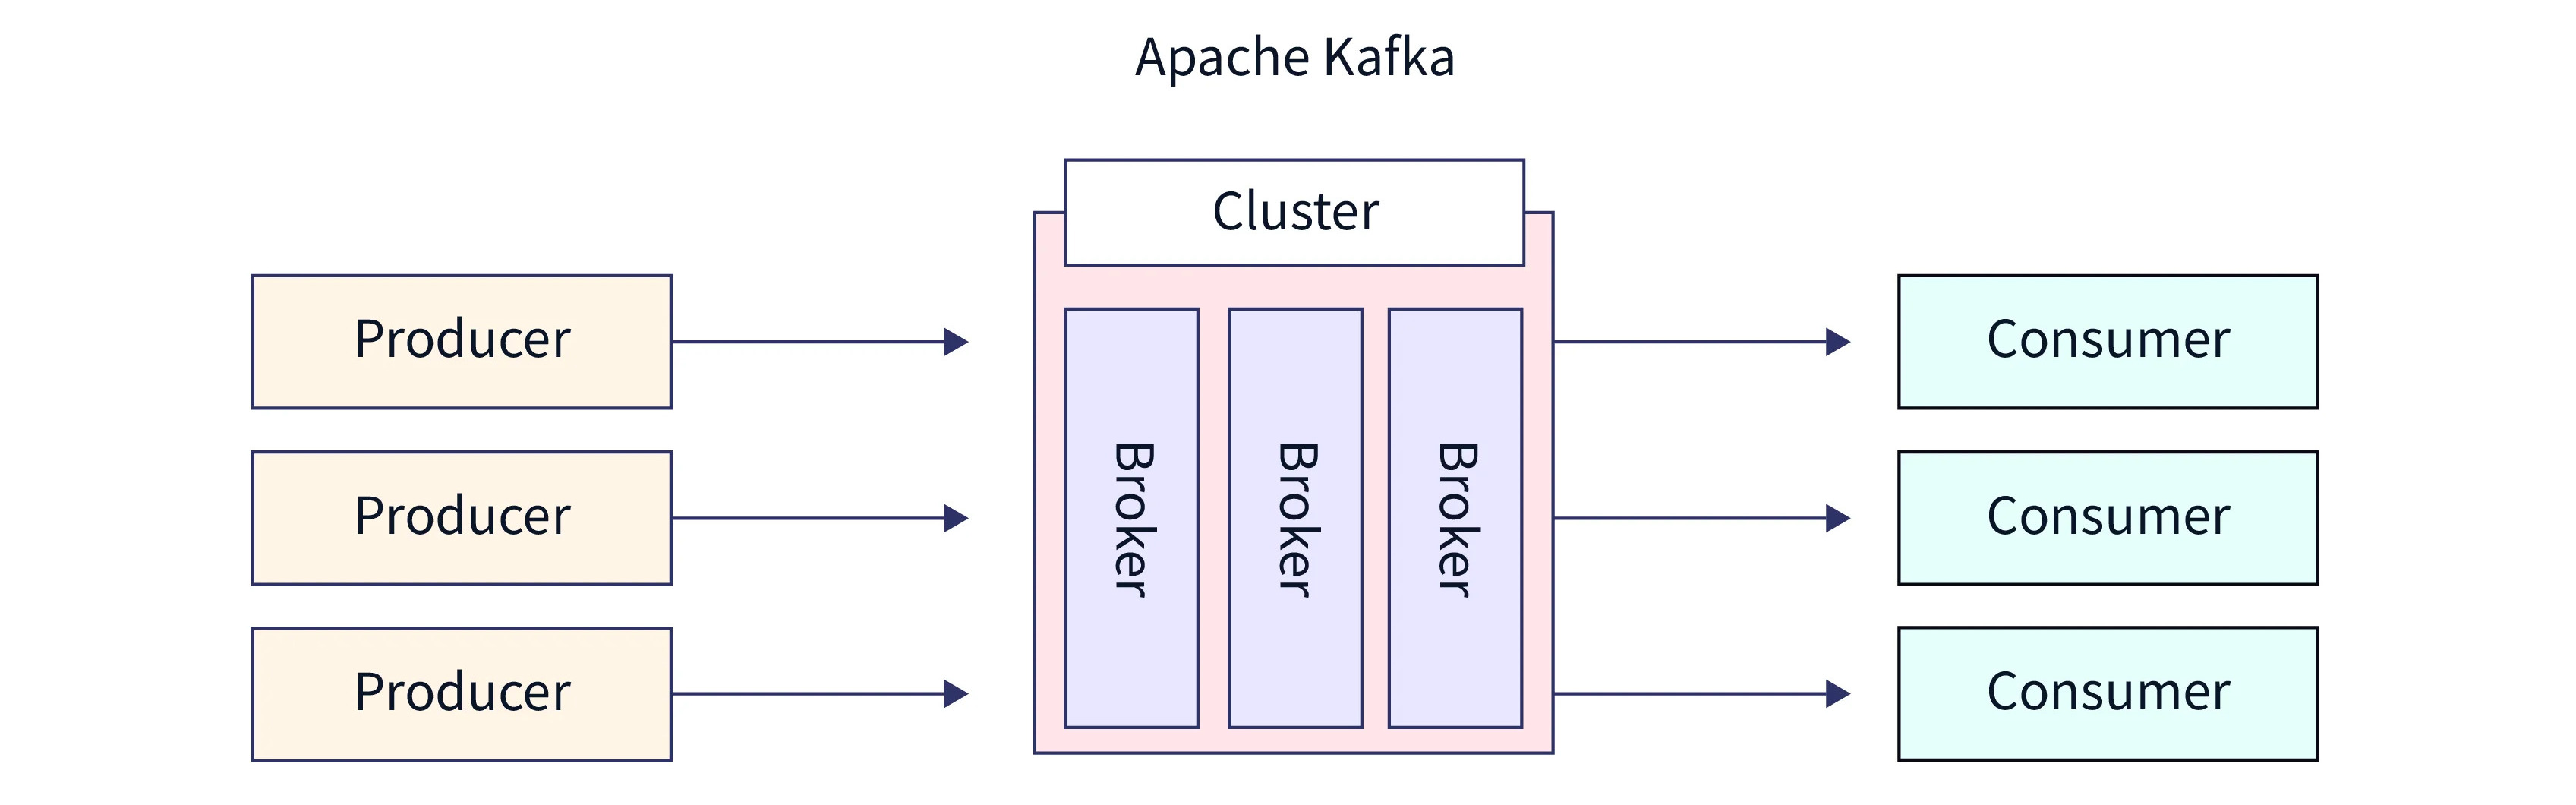
\includegraphics[width=\textwidth]{images/kafka/cluster.jpg}
    \caption{Kafka Cluster}
    \label{fig:kafka_cluster}
\end{figure}
% dovrei citare la fonte della figura https://www.scaler.com/topics/kafka-cluster/

\subsection{Topic}
\label{subsec:kafka_topics}

Un \textit{Kafka Topic} è un database ad eventi, al posto di pensare in termini di oggetti, si pensa in termini di eventi.
Diversi microservizi possono consumare o pubblicare sullo stesso \textit{Topic}, similmente ad un \texttt{Message Broker} infatti i \textit{Topic} sono \textit{multi-producer} e \textit{multi-subscribers}.
A differenza di un \texttt{Message Broker} però un \textit{Topic} può mantenere dei record in maniera sicura per una durata di tempo indefinita, come se fosse un database.Gli \textbf{Eventi} infatti non sono eliminati dopo esser stati letti da un \textit{Consumer},
il tempo di mantenimento di un record può essere configurato in modo da stabilire un equilibrio tra quantità di dati salvati e efficienza delle elaborazioni, dato che ad un numero maggiore di record corrisponde un tempo di elaborazione maggiore.\\\\
I \textit{Topic} sono partizionati per permettere high-availability, fault-tollerance e soprattutto consentire la lettura/scrittura in parallelo.
Infatti ogni \textit{Topic} è distribuito tra vari \textit{buckets}, che si trovano nei \texttt{Kafka Brokers}.
Eventi definita dalla stessa \textit{Key} sono scritti nella stessa partizione e \textit{Kafka} garantisce che qualsiasi \textit{Consumer} iscritto a tale partizione leggerà gli eventi nello stesso ordine in cui sono stati scritti.
Come citato prima il partizionamento permette anche la scrittura in parallelo, infatti se la partizione su cui due \textit{Producer} scrivono è differente e possibile effettuare l'operazione senza doversi preoccupare dei problemi generati dalla scrittura concorrente, anche se il \textit{Topic} è il medesimo.
Un esempio di partizionamento è mostrato in figura \ref{fig:kafka_topic}
\begin{figure}[htbp]
    \centering
    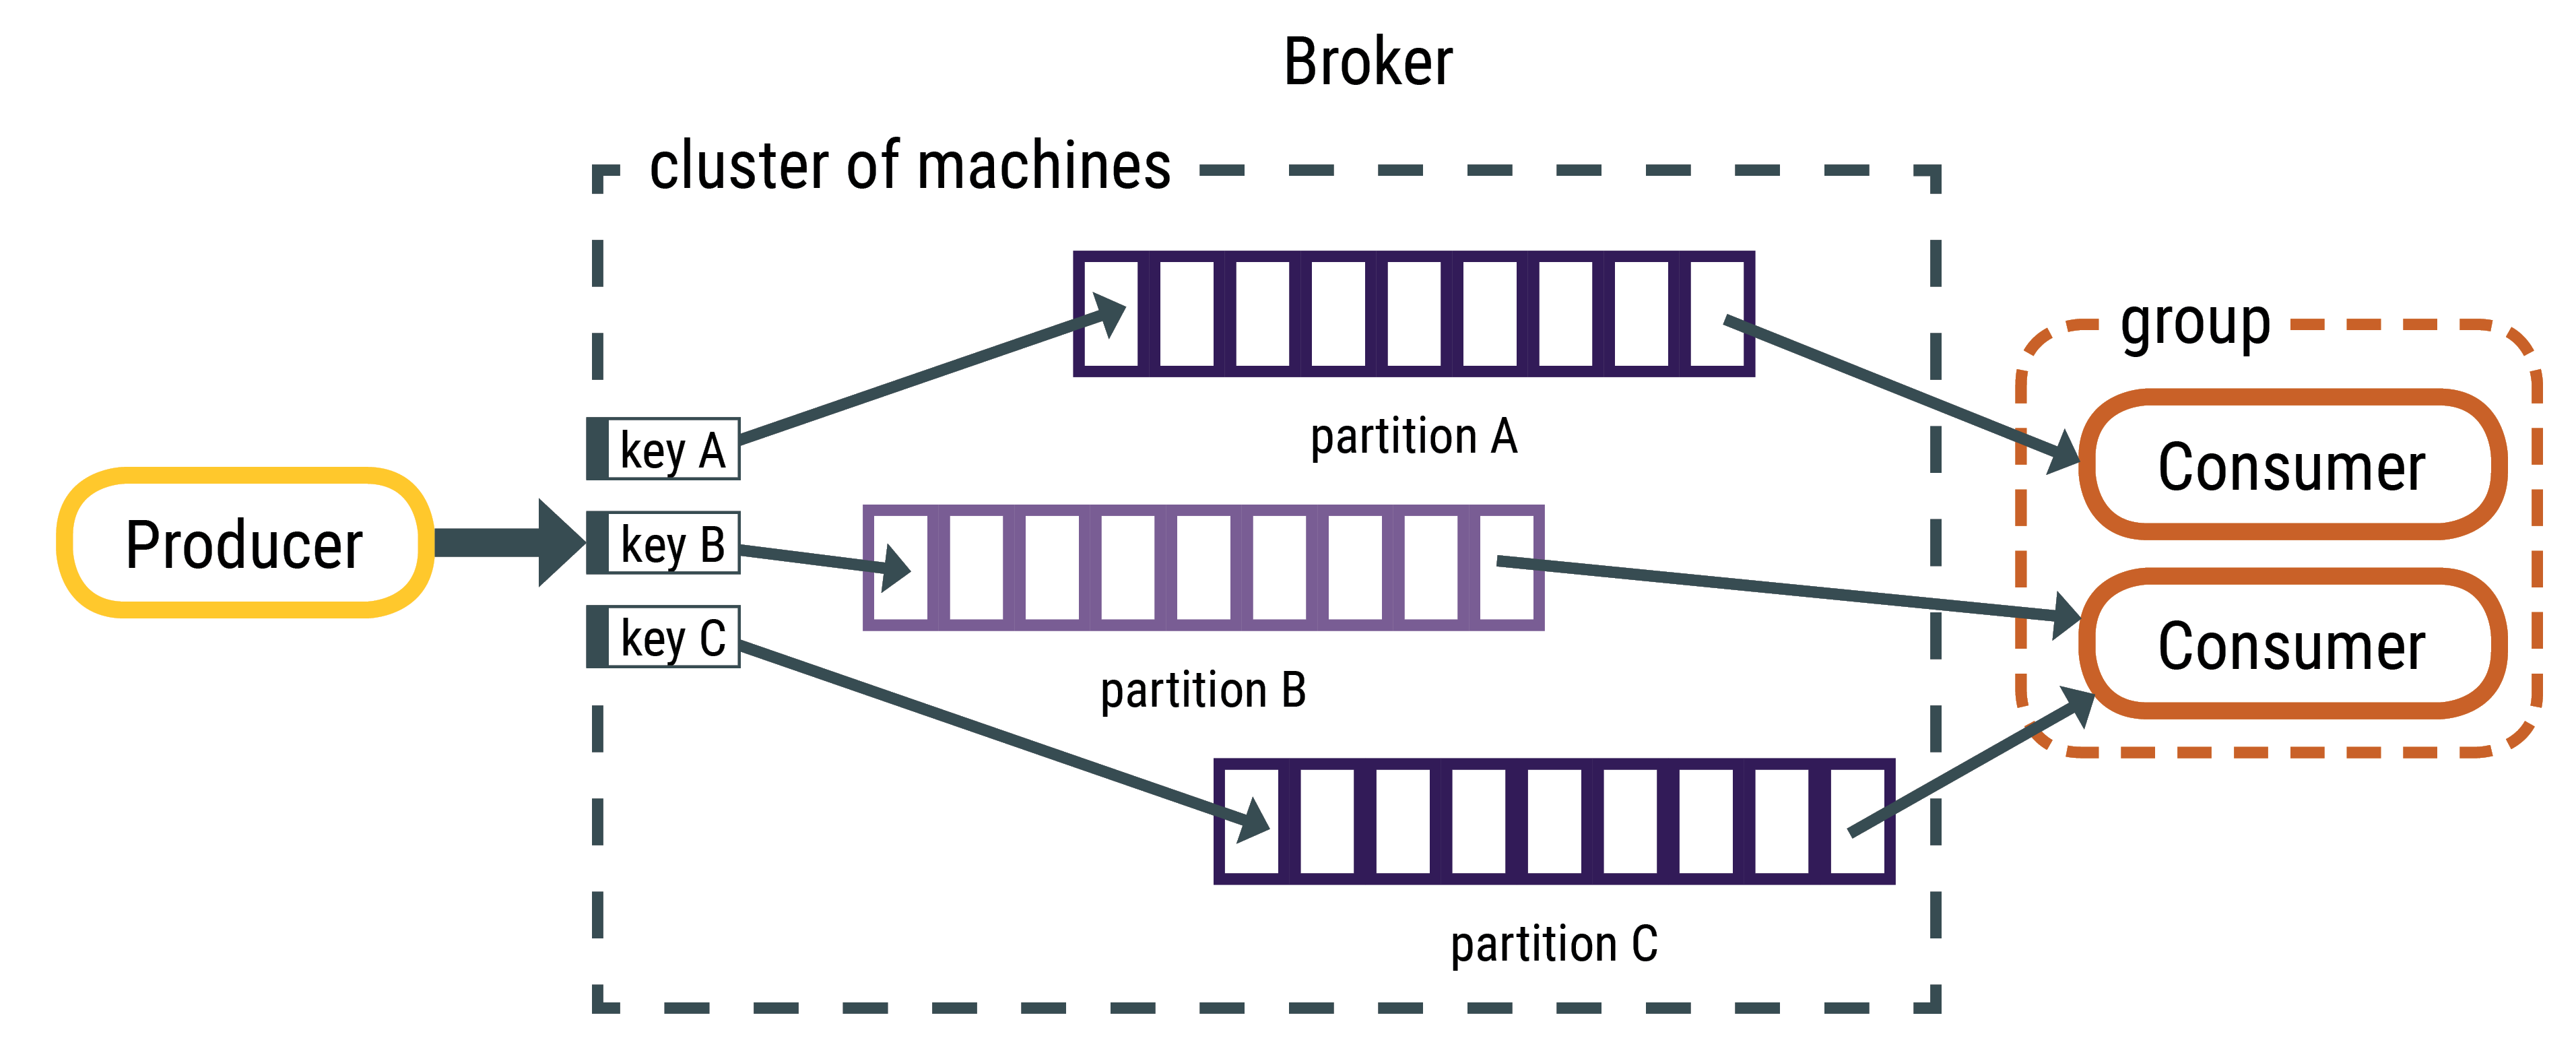
\includegraphics[width=0.9\textwidth]{images/kafka/topic.png}
    \caption{Partizionamento Kafka Topic}
    \label{fig:kafka_topic}
\end{figure}
%https://docs.datastax.com/en/kafka/doc/kafka/kafkaHowMessages.html

\newpage
\subsection{Clients}
\label{subsec:kakfa_clients}
I \texttt{Consumers} ed i \texttt{Producers}, insieme ai \textit{Topics}, sono gli elementi alla base del funzionamento di \textit{Kafka}.
Il \textit{Cluster Kafka} composto dai vari \textit{Brokers} svolge il ruolo di \textbf{Server}, mentre i \texttt{Consumers} ed i \texttt{Producers} fungono da \textbf{Clients},
collegandosi al cluster e interagendo con i dati presenti sui \textit{Topics}.
I \textit{Clients} sono i componenti che si occupano di implementare la logica di business e sono quindi interamente scritti dallo sviluppatore che sfruttera le due API messe a disposizione da Kakfa,
\textit{Consumer API} e \textit{Producer API}

\subsection{Streams}
\label{subsec:kafka_streams}
\texttt{Kafka Streams} è una API per processare eventi su un \texttt{Topic Kafka} (filtrare, trasformare, aggregare, ...).
Ad esempio se volessi sapere quanti ordini di trasporto sono stati spediti oggi, potrei fare un filtro per data e poi un count,
quello che il \texttt{Kafka Stream} fornirà in output sarà un altro flusso di dati filtrato, che potrò salvare su un nuovo \texttt{Topic} o in un database.\\
Nascono con l'intenzione di "astrarre" tutte le operazioni di basso livello quali la lettura o la scrittura su un \textit{Topic}, permettendo allo sviluppatore di preoccuparsi solamente di come i dati devono essere modificati, senza dover scrivere codice per ottenerli o ripublicarli.
In pratica qualsiasi operazione implementabile tramite \texttt{Kafka Streams} sarebbe allo stesso modo implementabile da un microservizio che legge da un \textit{Topic}, elabora i dati e li riscrive su un \textit{Topic}(lo stesso o un altro), ma grazie agli \texttt{Streams} si possono delegare le operazioni di collegamento con il \texttt{Kakfka Cluster} e concentrarsi solamente sull'elaborazione dei dati.
L'utilizzo dei \texttt{Kafka Streams} ha i seguenti vantaggi:
\begin{itemize}
    \item Efficienza: Il tipo di computazione è per-record, cioè ogni dato pubblicato sul \textit{Topic} a cui lo \texttt{Stream} è collegato viene subito processato. Non c'è bisogno di effettuare "batching", cioè richiedere i dati ad intervalli di tempo regolari ed elaborare solo i dati giunti in tale intervallo. Il sistema può lavorare quasi in tempo reale.  
    \item Scalabilità: Gli \texttt{Stream} sono scalabili e fault-tollerant. Essendo \textit{Kafka} pensato per essere un sistema distribuito anche gli \texttt{Streams} sono pensati per essere scalati e distribuiti, se si creano diverse istanze dello stesso \texttt{Stream} queste collaboreranno automaticamente suddividendosi il carico computazionale.
    \item Riuso del codice: si utilizza una chiamata all API al posto di riscrivere lo stesso codice per differenti microservizi.
\end{itemize}

\subsection{Connector}
\label{subsec:kafka_connectors}
I \texttt{Connectors} sono particolari tipi di \texttt{Consumers/Producers}, il cui scopo è mettere in comunicazione \textit{Kafka} con altri sistemi.
I \texttt{Connectors} producono flussi di eventi partendo da dati ricevuti da un altro sistema (\textit{Source Connector}), oppure consumano da un topic e inviano i dati letti ad una applicazione esterna(\textit{Sink Connector}).
Per esempio un \texttt{Connector} ad un database relazionale potrebbe catturare tutte le operazioni effettuate su una tabella e generare un flusso di eventi in cui ogni evento corrisponde ad un cambiamento.\\
Similmente ai \textit{Kafka Streams} (\ref{subsec:kafka_streams}) i principali vantaggi di utilizzare un \texttt{Connector} piuttosto che scrivere da se il codice per svolgere lo stesso compito sono
\textbf{efficienza}, \textbf{scalabilità} e \textbf{riuso del codice}.
Inoltre sono presenti diversi repository online dove trovare \texttt{Connector} già pronti, sviluppati dalla community o dagli sviluppatori delle applicazioni esterne (sqlserver, JDBC, Amazon S3),
uno dei più diffusi è il \texttt{confluent-hub} https://www.confluent.io/product/connectors/ \todo{questo deve diventare un link o essere spostato in bibliografia}

\newpage
\section{Debezium}
\label{sec:debezium_overview}
\textit{Debezium is an open source distributed platform for change data capture. Start it up, point it at your databases, and your apps can start responding to all of the inserts, updates, and deletes that other apps commit to your databases.}\cite*{debeziumwebsite}\\\\
\texttt{Debezium} è una piattaforma distribuita open source per la cattura dei dati di modifica, permette di catturare le operazioni di modifica effettuate su un database (\textit{insert, update e delete}) e di trasformarle in eventi.
Nativamente tutti i più comuni database sono supportati, tra cui \textit{MySQL, PostgreSQL, MongoDB, SQL Server, Oracle, ...}.\\\\
\texttt{Debezium} è costruito sulla base di \textit{Apache Kafka}, di conseguenza è facilmente integrabile con esso.
Ci sono infatti due modi per utilizzare questa piattaforma: come un sistema distriubuito a se stante oppure tramite un \texttt{Kafka Connector}(\ref{subsec:kafka_connectors}).
Il primo modo presenta tutti i vantaggi di un sistema distribuito, come la scalabilità e la fault-tollerance, ma ha un costo in termini di risorse, di configurazione e di gestione.
In questo modo è inoltre possibile consumare gli eventi prodotti tramite un qualsiasi sistema esterno, non si è obbligati ad utilizzare \textit{Kafka}.\\
Se invece si ha già una infrastruttura già basata su \textit{Kafka} è molto più conveniente utilizzare \texttt{Debezium} come \texttt{Connector}, con un considerevole risparmio di risorse e di tempo.  

\newpage
\section{Apache Flink}
\label{sec:flink_overview}
\textit{Apache Flink is a framework and distributed processing engine for stateful computations over unbounded and bounded data streams. Flink has been designed to run in all common cluster environments, perform computations at in-memory speed and at any scale.}\cite*{flinkwebsite}\\\\
\textit{Apache Flink} è sia un framework che un motore di elaborazione distribuito per la computazione di flussi di dati (\texttt{streams)}), \textit{bounded} e \textit{unbounded}.
Può essere utilizzato per elaborare dati in tempo reale, ma anche per elaborare grandi quantità di dati in batch.
Fornisce sia una API per la creazione di applicazioni di elaborazione di dati, sia un \textit{runtime} environment distribuito per eseguirle,
per questo motivo si può considerare sia un \textit{framework} che un \textit{motore di esecuzione}.
Come anticipiato i tipi di dato trattato sono sempre \texttt{streams} che possono essere:
\begin{itemize}
    \item \textbf{Unbounded}: un flusso di dati che non ha un inizio o una fine, come ad esempio un flusso di eventi generati da un sensore.
    \item \textbf{Bounded}: un flusso di dati con un inizio e una fine, come ad esempio un file o una tabella di un database.
\end{itemize}
Sui flussi \textit{Bounded} possono essere eseguite tutte le operazioni eseguibili sui flussi \textit{Unbounded}, ma non viceversa.
Per fare ciò bisogna ricorrere a delle operazioni di \textit{windowing}, cioè dividere il flusso in finestre (temporali o di conteggio 
\footnote{Per \textit{finestra di conteggio} si intende una finestra che contiene un numero fisso di elementi, ad esempio una finestra di 100 elementi.
In inglese si parla di \textit{count window}. maggiori informazioni nella sezione \textit{Windowing} \ref{subsec:flink_windowing}}
) e poi eseguire le operazioni su queste finestre.

\subsection{Statefull stream processing}
\label{subsec:flink_statefull_processing}
\textit{Flink} può svolgere operazioni che richiedono il mantenimento di uno stato, cioè un insieme di informazioni riguardanti gli eventi passati.
Semplici esempi di elaborazioni che richiedono uno stato sono: la ricerca di un pattern, il calcolo di una media (mobile se si parl di \textit{Stream Unbounded}), il calcolo di una somma, etc \dots
\textit{Flink} sfrutta lo stato anche per garantire la \textit{fault-tollerance}, cioè la capacità di ripristinare il sistema in caso di guasto.\\\\
Il metodo più comune con cui una applicazione \textit{Flink} sfrutta lo \textit{Statefull processing} è tramite l'uso di \textit{Keyed Stream}.
Operando su un \texttt{DataStream} può essere effettuata una operazione di \texttt{keyBy(key)}, dove \textit{key} è un qualsiasi oggetto java (POJO) che implementa il metodo \texttt{hashCode()}.
Tale operazione permette di raggruppare gli eventi in base ad una chiave, in modo che tutti gli eventi con la stessa chiave appartengano alla stessa partizione logica.
Si ottiene quindi un \texttt{KeyedStream} su cui è possibile eseguire operazioni di \textit{statefull processing}, 
il seguente codice di esempio mostra come calcolare la somma di un \texttt{KeyedStream} di ogetti composti da una chiave (\textit{f0}) e un valore(\textit{f1}):\\
\begin{code}
    \inputminted{java}{listings/keyed-stream.java}
    \caption{Esempio di operazione statefull su un KeyedStream}
    \label{lst:keyed_stream}
\end{code}
Oltre ad essere necessario per mantenere uno stato il partizionamento tramite chiave permette anche di parallelizzare le operazioni, 
dato che ci assicura non ci saranno conflitti tra le operazioni eseguite su partizioni diverse.
Nell'esempio precedente (listing \ref{lst:keyed_stream}) la somma potrebbe venire calcolata in parallelo per ogni chiave, dato che lo stato mantenuto dal sistema,
che corrispone semplicemente alla variabile \texttt{accumulator}, non viene mai acceduto durante la computazione di un dato avente un'altra chiave, posto naturalmente che si abbia a disposizione sufficienti risorse computazionali.
Il discorso di come \textit{Flink} gestisca le risorse è approfondito nella sezione \ref{subsubsec:flink_Task_slots}.

\todo{parlare del checkpointing?}

\subsection{Windowing}
\label{subsec:flink_windowing}
Alcune elaborazioni richiedono di operare su un sottoinsieme di dati, soprattutto quando si tratta di flussi di dati \textit{Unbounded}.
Ad esempio se si volesse calcolare la media di un flusso di dati, sarebbe necessario calcolare la media solo sui dati arrivati in uno specifico intervallo, 
non è possibile calcolare la media su tutti i dati del flusso dato che il flusso non ha un inizio o una fine.
Il \textit{windowing} è una tecnica di elaborazione di flussi di dati che permette di dividere un flusso in finestre,
su cui poi eseguire operazioni di aggregazione o riduzione.
Tornando all'esempio della media, si potrebbe dividere il flusso in finestre temporali di 1 minuto e poi calcolare la media su ciascuna finestra.\\\\
Le finestre possono essere \textit{temporali} o \textit{di conteggio}, le prime sono divise in base al tempo, ad esempio una finestra di 1 minuto,
le seconde in base al numero di elementi, ad esempio una finestra di 100 elementi.
Rispettando questa distinzione si possono avere altri 3 tipi di finestre:
\begin{itemize}
    \item \textbf{Tumbling Window}: una finestra temporale o di conteggio che non si sovrappone ad altre finestre, ad esempio una finestra di 1 minuto.
    \item \textbf{Sliding Window}: una finestra temporale che si sovrappone ad altre finestre, ad esempio una finestra di 1 minuto che si sposta di 30 secondi ad ogni nuovo evento.
    \item \textbf{Session Window}: una finestra temporale che si basa su un intervallo di tempo inattivo, ad esempio una finestra di 1 minuto che si chiude quando non ci sono eventi per 5 secondi.
    Come le sliding window anche le session window si possono sovrapporre.
\end{itemize}
Un esempio dei vari tipi di finestra è mostrato in figura \ref{fig:flink_window}

\begin{figure}[htbp]
    \centering
    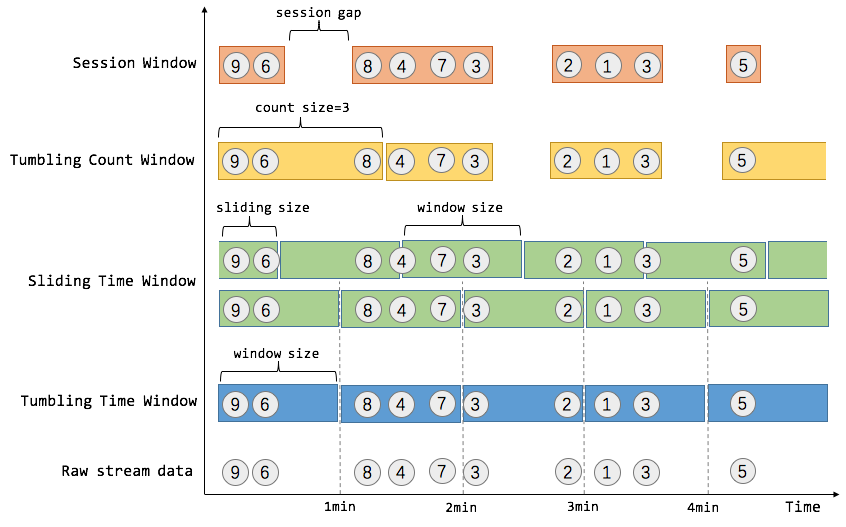
\includegraphics[width=\textwidth]{images/flink/windows.png}
    \caption{Tipi di finestra}
    \label{fig:flink_window}
\end{figure}
%TODO: citare la fonte dell'immagine https://datafibers-community.github.io/blog/2019/10/05/2019-10-05-flink-windows-explained/

\subsubsection{Wartermarks}
\label{subsubsec:flink_watermarks}
Legato al concetto di finestra temporale è il concetto di \textit{Watermark}, un \textit{Watermark} è un marcatore temporale che indica il punto in cui non ci saranno più eventi precedenti.
Nascono dalla necessità di misurare il tempo quando si lavora con \textit{finestre temporali} dato che l'operatore \textit{finestra} ha bisogno di essere notificato
quando è passato più tempo di quanto specificato ed è ora che la finestra si chiuda (non accetti più eventi) ed inizi la computazione.\\\\
I \textit{watermarks} vengono gestiti da \textit{Flink} come se fossero normali eventi, sono inseriti all'interno del flusso di eventi e contenfono un timestamp \textit{t}.
quando il \textit{Watermark} con timestamp $t$ raggiunge l'operatore finestra l'assunzione implicita è che non ci dovrebbero più arrivare elementi con timestamp $t'$ tali per cui $t' \leq t$.
Cioè eventi verificatisi "prima" del tempo $t$ del \textit{watermark}.
Questo strumento non sembra molto utile finchè si considerano flussi di dati ordinati ma diventa fondamentale se il flusso su cui stiamo operando presenta eventi
non ordinati (rispetto al timestamp).
Situazione che si verifica di frequente quando si ha a che fare con sistemi complessi e distribuiti dove non è garantito che gli eventi 
giungano al sistema di elaborazione mantenendo l'ordine con cui sono avvenuti.
Un esempio di flusso con eventi non ordinati ed il relativo uso dei \textit{watermarks} è mostrato nella figura \ref{fig:watermark}\\\\
\begin{figure}[htbp]
    \centering
    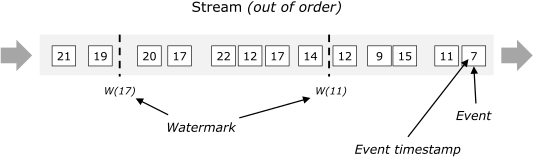
\includegraphics[width=0.8\textwidth]{images/flink/watermark_out_of_order.png}
    \caption{Watermarks in out-of-order stream}
    \label{fig:watermark}
\end{figure}
Nel caso di eventi fuori ordine si possono impostare le \textit{finestre} in modo che permettano un "ritardo" nell'arrivo di alcuni eventi anche dopo che il \textit{watermark} ha raggiunto la finestra.
Gli eventi in ritardo sono formalmente definiti come gli eventi aventi $t' \leq t$ ma che giungono alla \textit{finestra} dopo l'arrivo del \textit{watermark} e possono essere gestiti in diversi modi.
Tra i più comuni abbiamo la possibilità di reindirizzarli in un apposito flusso (\textit{side output}) oppure di rielaborare tutti i dati nella \textit{finestra} scartando la precendente computazione (\textit{firing})

\subsection{Flink Cluster}
\label{subsec:flink_cluster}
Un \textit{Flink Cluster} è penasto per essere eseguito in un ambiente distribuito, come ad esempio un \textit{Hadoop YARN} o \textit{Kubernetes},
ma non è limitato a ciò, può essere eseguito anche in un ambiente \textit{standalone} oppure si può sfruttare solo la API di Flink senza dover necessariamente eseguire un \textit{Cluster}.
\begin{figure}[htbp]
    \centering
    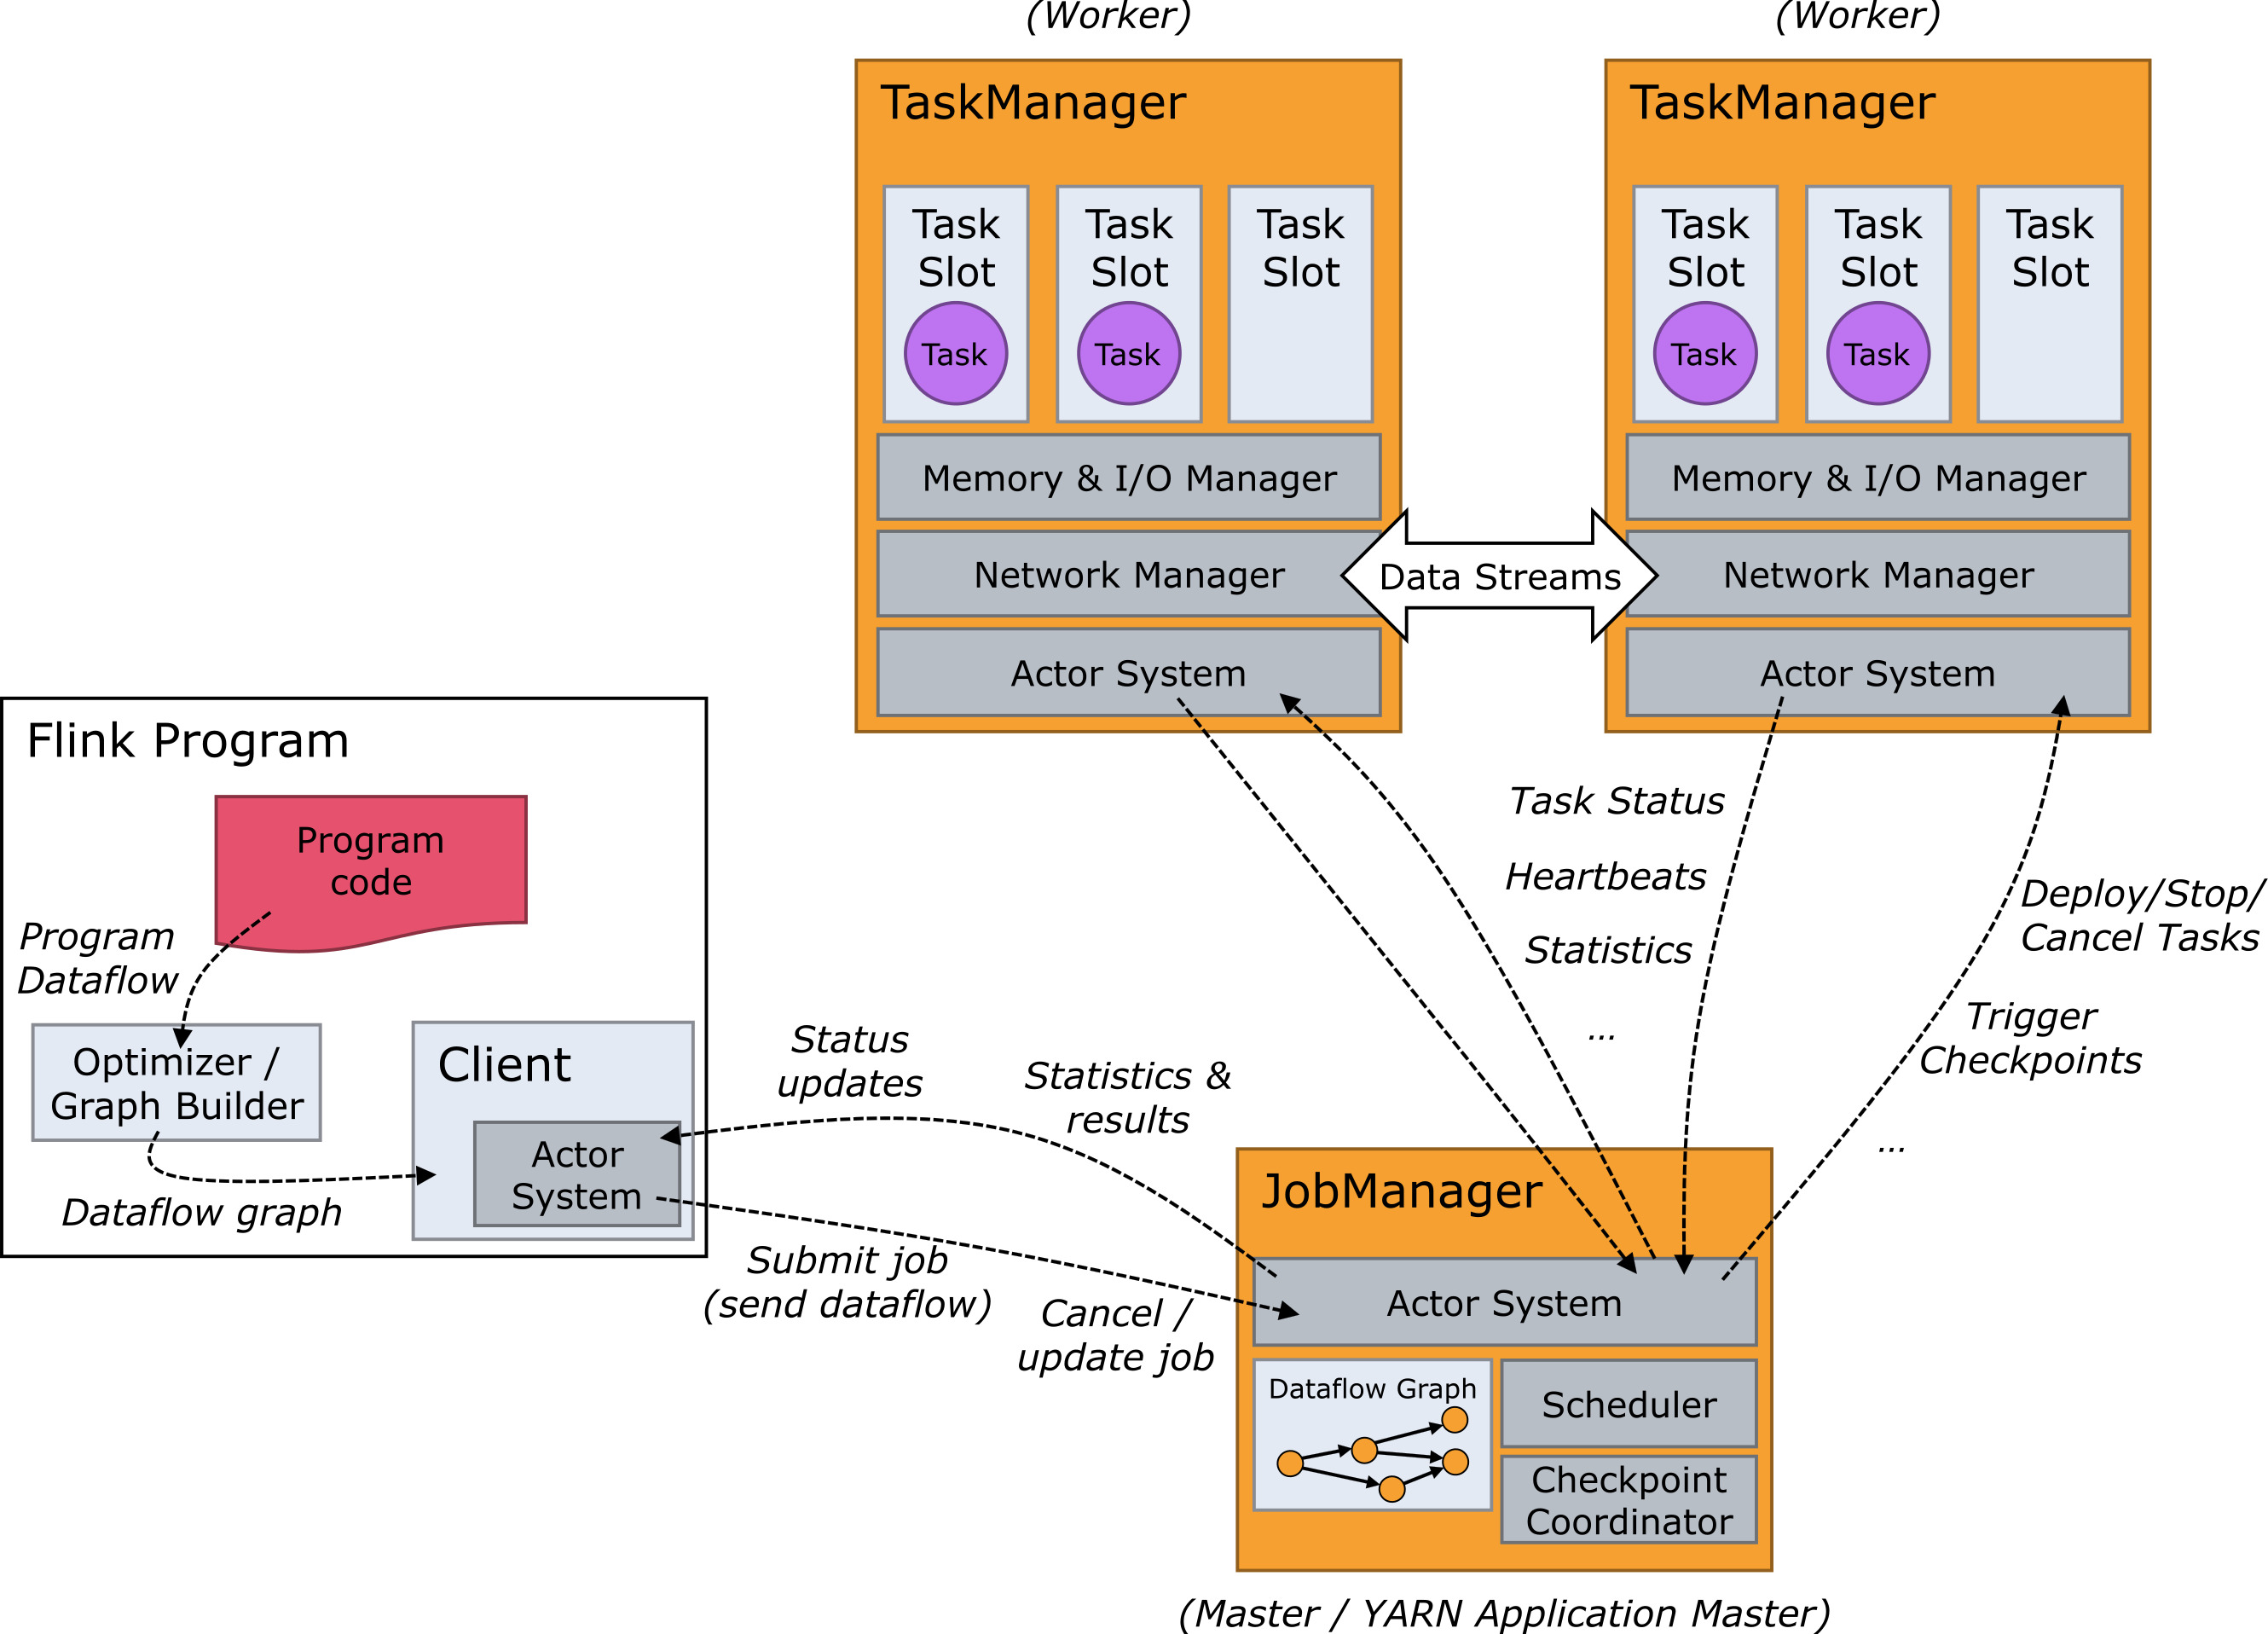
\includegraphics[width=\textwidth]{images/flink/cluster.jpg}
    \caption{Flink Cluster}
    \label{fig:flink_cluster}
\end{figure}
\\Il \textit{runtime environment} di Flink è composto da due tipi di processi: i JobManager ed i TaskManager.
\begin{itemize}
    \item \textbf{JobManager}: è il master del \textit{Cluster}, si occupa di coordinare il lavoro dei \textit{TaskManager} decidendo quando eseguire un Task,
    gestire gli errori in fase di esecuzione ed effettuare checkpointing 
    \footnote{Il meccanismo di checkpoint è una strategia di \textit{fault tolerance} basata sul mantenere degli snapshots di vari componenti del sistema
    per poterlo ripristinare in caso di guasto}.
    Le principali responsabilità del \textit{JobManager} sono due: la gestione delle risorse e la gestione dei job.
    \begin{enumerate}
        \item \textbf{Gestione delle risorse}: il \textit{JobManager} gestisce i \textbf{Task Slots} (sezione \ref{subsubsec:flink_Task_slots}) dei \textit{TaskManager}, cioè le risorse computazionali.
        Se l'ambiente di esecuzione è distribuito (come ad esempio \textit{YARN} o \textit{Kubernetes}) il \textit{JobManager} può richiedere di avviare nuove istanze di \textit{TaskManager} in base alle necessità.
        \item \textbf{Gestione dei job}: il \textit{JobManager} si occupa di ricevere i job da eseguire, di distribuirli tra i \textit{TaskManager} e di monitorarne l'esecuzione.
        Inoltre fornisce una REST API ed una interfaccia web per monitorare lo stato del cluster e per ricevere nuovi jobs.
    \end{enumerate}
    C'è sempre almeno un \textit{JobManager}. Una configurazione \textit{Hig-Availability} potrebbe avere più \textit{JobManager}, di cui uno è sempre il leader e gli altri sono in standby.
    \item \textbf{TaskManager}: sono i worker del \textit{Cluster}, si occupano di eseguire i Task e di ricevere e inviare i dati.
    La più piccola unità di esecuzione in un TaskManager è un \textbf{Task Slots} (sezione \ref{subsubsec:flink_Task_slots}).
    Il numero di slot di Task in un TaskManager indica il numero di Task eseguibili in parallelo.
\end{itemize}

\subsubsection{Task Slots}
\label{subsubsec:flink_Task_slots}
Per comprendere il concetto di \textit{Task Slot} è necessario comprendere come viene gestito il \textit{parallelismo} in \texttt{Flink}.    
Un programma scritto tramite l'API di \texttt{Flink} non viene eseguito sequenzialmente, ma viene diviso in sottoprocessi che possono essere eseguiti in parallelo.
Ad esempio un semplice programma che riceve dei dati, li filtra e li salva su un database potrebbe essere diviso in tre sottoprocessi: ricezione, filtro e scrittura.
Questi tre sottoprocessi sono chiamati \textit{Task} e possono essere, parzialmente, eseguiti in parallelo.\\
Inoltre, come anticipato nella sezione \ref{subsec:flink_statefull_processing}, una operazione di \texttt{KeyBy()} suddivide uno stream in partizioni di dati
indipedenti tra loro, quindi tutte le operazioni su questi dati possono essere eseguite in parallelo.
Potenzialmente potremmo eseguire la computazione di questi dati dedicando un \textit{Task} ad ogni partizione, cioè per ogni \textit{key} presente nello stream,
ottenendo così il massimo parallelismo possibile.
Qualora non si abbia a disposizione sufficienti risorse computazionali per dedicare ad ogni partizione un \textit{Task} il \texttt{Flink runtime environment} 
automaticamente aggregherà più partizioni in un cosiddetto \textbf{Key Group} che verrà trattato come una qualsiasi altra partizione.
\\\\
Ogni \texttt{TaskManager} è sostanzialmente un processo che esegue la JVM ed il codice, quindi può eseguire uno o più sottoprocessi in diversi \textit{threads}.
Ogni \texttt{Task Slot} rappresenta un sottoinsieme di risorse computazionali di un \texttt{TaskManager}.
Ad esempio un \texttt{TaskManager} con 3 \texttt{Task Slot} dedicherà 1/3 delle sue risorse a ciascun \texttt{Task Slot}.
Più \texttt{Task Slot} si hanno a disposizione, più \texttt{Task} si possono eseguire in parallelo, ma anche meno risorse si avranno a disposizione per ciascun \texttt{Task}.
Inoltre se due \texttt{Task} operano sugli stessi dati è possibile effettuare \textit{slot sharing}, cioè permettere a due \texttt{Task} di condividere un \texttt{Task Slot}, limitando il parallelismo ma riducendo il consumo di memoria.
Come si può vedere nell'immagine \ref{fig:flink_slots} dove i \texttt{Task} \textit{Source} e \textit{Map} condividono un \texttt{Task Slot}.
\begin{figure}[htbp]
    \centering
    \includegraphics[width=\textwidth]{images/flink/Tasks_slots.jpg}
    \caption{Task Slots sharing}
    \label{fig:flink_slots}
\end{figure}